%!TEX root = ../report.tex

% 
% Architecture
% 

\section{Architecture}

%introduction
This is the proposed solution to solve the need of a refactoring tool designed for unexperienced users.
%A refactoring tool that would suit an unexperienced programmer who is learning how to program is needed.
The choice of language and environment is important, so it was chosen the Racket programing language and the DrRacket environment.
Racket is a dynamic language that is known of being used as an introductory programming course in schools around the world. 
Racket also has an IDE, DrRacket that is a pedagogic environment \cite{drscheme_pegadogy} and it also supports development and extension of other programming languages \cite{tobin2011languages} and recently it has an implementation of python \cite{ramos2014implementation}.
Besides that, DrRacket only has one refactoring operation, that is the rename.
That will motivate the unexperienced programmers to start using tool assisted refactoring operations and DrRacket seams to be the ideal candidate to have that refactoring tool.


%use cases: To validate the architecture.
\subsection{Refactoring Operations}
%Das operacoes para a refactoring tool vamos falar particularmente destas, ou por exemplo destas.
The refactoring tool consists in a set of refactoring operations.
This describes some of the refactoring operations desired and their use.
%introduce the validate cases xD

% rename improved
\subsubsection{Rename}
\label{ssub:Rename}
%this is a refactoring for racket
is the most used refactoring operation and it is indispensable to any refactoring tool.
DrRacket environment already has a rename operation, however the rename has a bug when renaming imported functions.
When renaming a imported function the original rename of DrRacket renamed the name of all the imported functions from the same file and it also renamed the name of the file imported.
This is not a correct refactoring, this makes the program syntactic incorrect because it renames the name of the file imported and DrRacket should only rename the function with the selected name, not every function from that file.
This situation may occur when using functions from other file, whether because there is a name conflict or it is better for the readability to rename that function name.
%After that, the user can call the methods exported like they were defined in the file.
%However those methods could have name collision or change it for a more adequate name. To do that the user would do a rename.


% extract-function
\subsubsection{Extract-function}

is a simple and very useful refactoring, and it is shown previously in this document that is one of the most used refactoring operations.

Extract-function is an important refactoring for unexperienced users since those users tend to create a big function that does all the work.

By having a mean to restructure the code, unexperienced programmers will be able to create programs with better quality.




\subsubsection{Move expression}

Move expression is also one of the most used refactoring operations.
This operation allows the user to move safely the expressions to the new location.



% add-prefix
\subsubsection{Add-prefix}
%this is a refactoring for racket only!
is a particular refactoring operation for Racket.
%When using two libraries that have functions with the same name there is a naming conflict.
%This happens when a programmer is using some functions from a library and then realizes that needs another function.
%The new function has the same name of one of the used functions and that creates a conflict error.
%The solution is to add a prefix for one of the imported libraries.

When there several functions are imported from several different libraries the code starts to became confusing because it is hard to remember where a specific function came from.
To solve that problem Racket as a prefix that can be added to the imported functions.
This prefix helps improving the readability of the code and therefore the quality.
That is really annoying because the user has to remember and change one by one all functions invocations.

The Add Prefix refactoring does all that for the user.
This is also useful when the name of the functions are similar, adding a prefix make it easier to distinguish between libraries.





\subsection{Structure}
%s-exp and def-uses-relationships

%An image will be awesome here
The architecture of the refactoring tool will consist in an AST and in the def-use-relations of the program to be refactored.
The information gathered in the AST and in the def-use-relations with some preconditions is enough to ensure the correctness of the refactoring operations.
The AST in the Racket programing language is composed of s-expressions. Because a program is a list of s-expressions.
DrRacket provides the def-use-relations which is an important help to do the refactoring operations. The def-use-relations are visually represented as arrows in the DrRacket.

\begin{figure}[htbp]
	\centering
	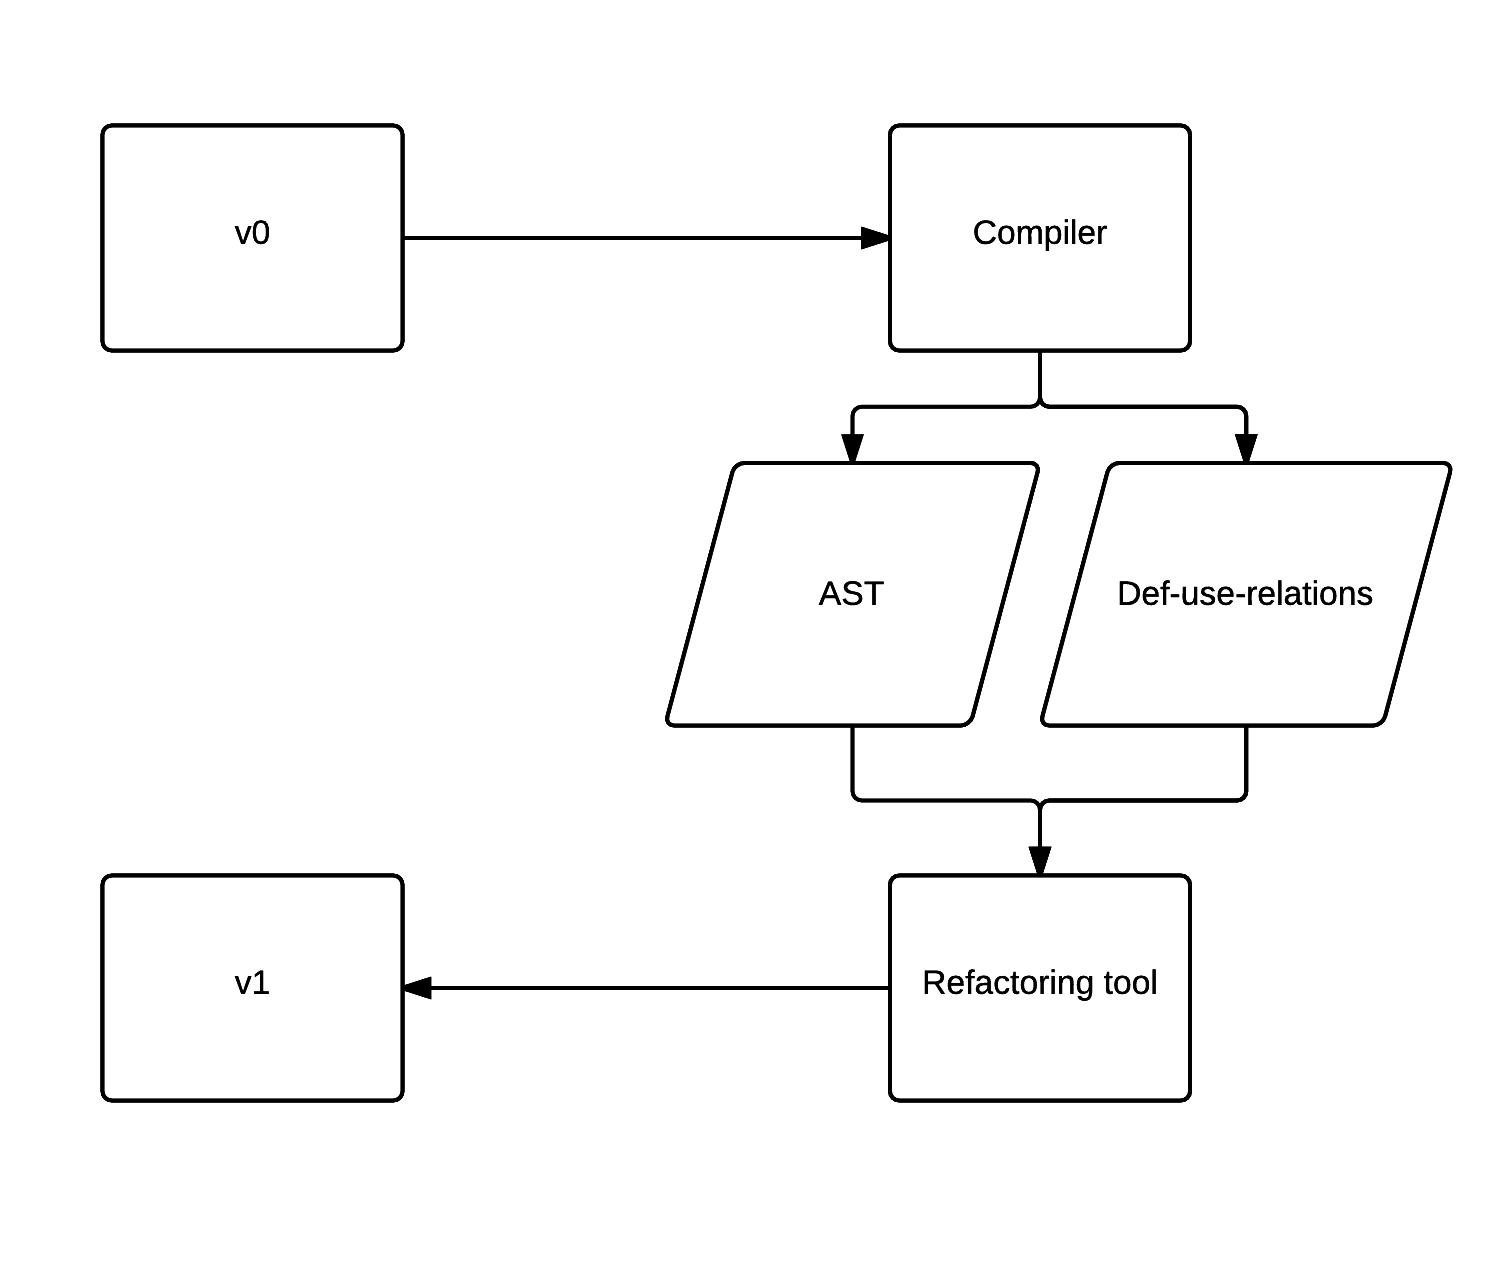
\includegraphics[width=0.95\textwidth]{img/arquitectura.png}
	\caption{Solution's architecture}
	\label{fig:architecture}
\end{figure}

As described in {\bf Figure~\ref{fig:architecture}}, the compiler generates the AST and the Def-use-relations of a program version. Then the refactoring tool uses that and some conditions to ensure that the refactoring is correct. After that it changes the program creating another version.

\subsection{Validation}
%In order to evaluate it was implemented a prototype in DrRacket.
In order to validate this architecture some refactoring operations were implemented. 
This allows to validate the architecture and have more trust in this architecture.
To do that it was only validated the refactoring operations that only used the def-use-relations.

\subsubsection{Extract-function}
The user selects the expressions that wants to extract and chooses a name for the new function as seen in {\bf Figure~\ref{fig:extractBefore}}.
Then the user pastes the result of the extraction where he thinks it's the best place for the function. {\bf Figure~\ref{fig:extractAfter}}.
The extract function refactoring could already paste the extracted function, however this way the user can choose the function's location.
\begin{figure}[htbp]
	\centering
	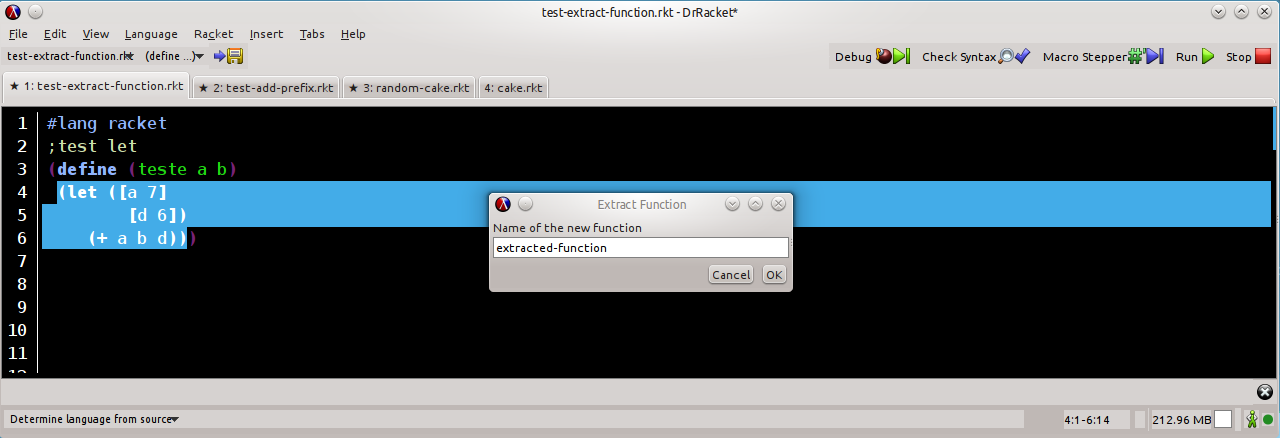
\includegraphics[width=0.95\textwidth]{img/extract1.png}
	\caption{Before the Extract function}
	\label{fig:extractBefore}
\end{figure}

\begin{figure}[htbp]
	\centering
	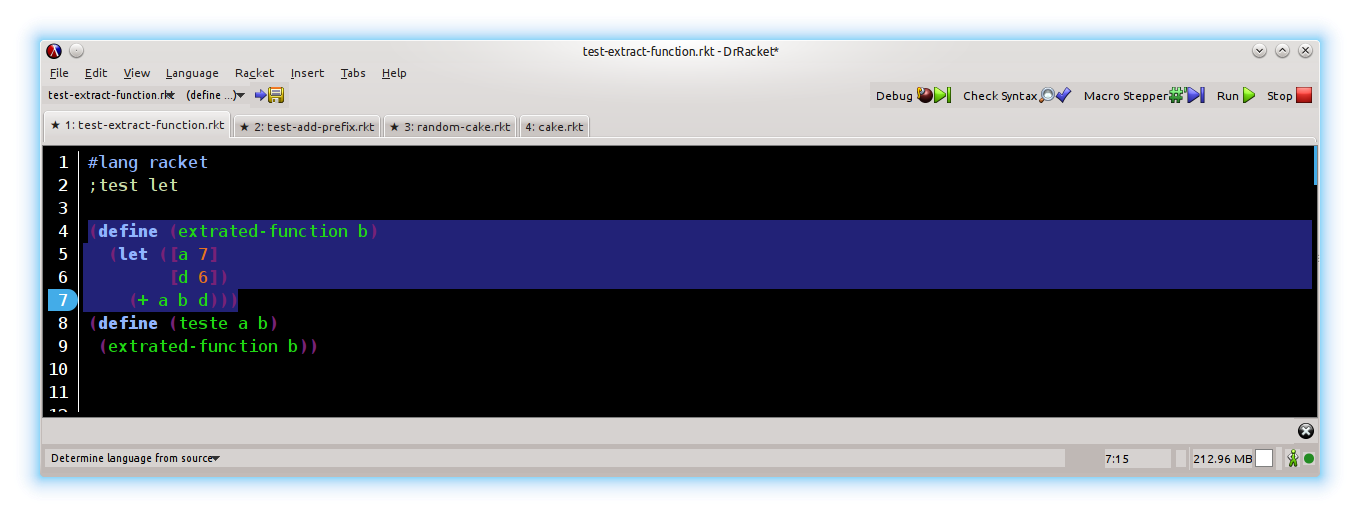
\includegraphics[width=0.95\textwidth]{img/extract2.png}
	\caption{After the Extract function}
	\label{fig:extractAfter}
\end{figure}

\subsubsection{Imported renames}
As explained in ~\ref{ssub:Rename} the DrRacket only refactoring operation the Rename has bugs when it has to rename imported functions.
This example regards only when renaming an imported function. The user selects the function that wants to be renamed, {\bf Figure~\ref{fig:renameBefore}} in this case the user chose ``print-cake'', then the user chooses the new name and the end result is shown in {\bf Figure~\ref{fig:renameAfter}}.
\begin{figure}[htbp]
	\centering
	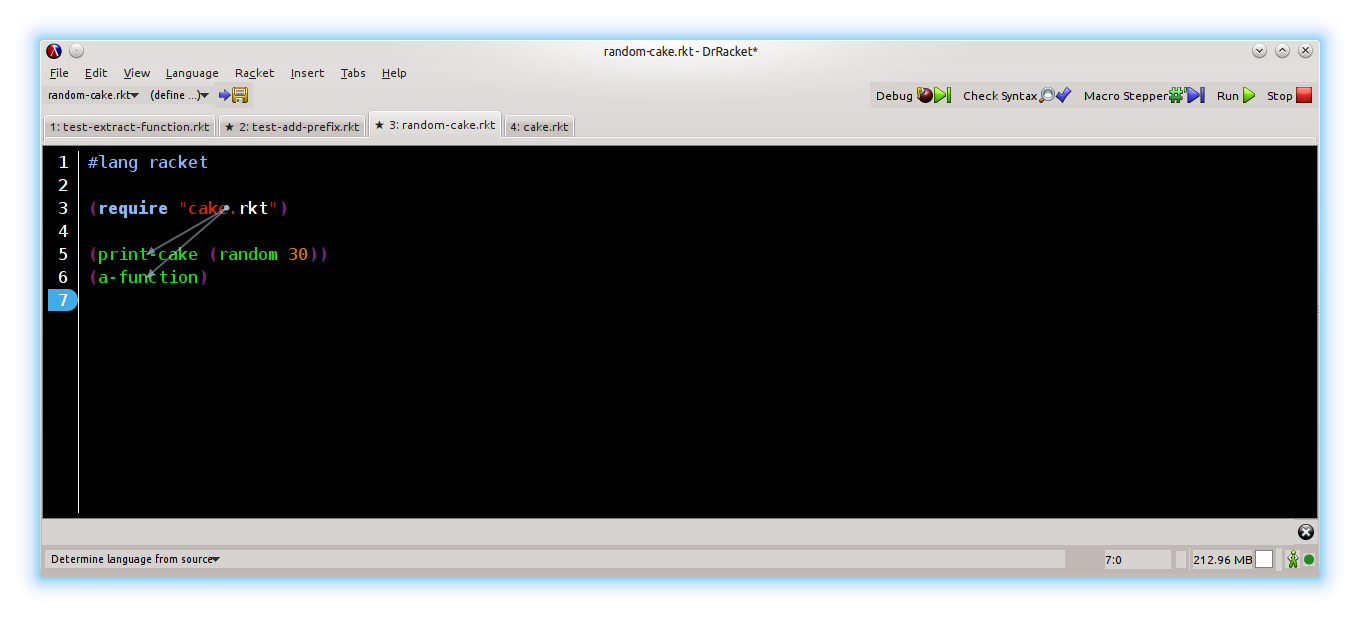
\includegraphics[width=0.95\textwidth]{img/rename1.png}
	\caption{Before the Rename}
	\label{fig:renameBefore}
\end{figure}

\begin{figure}[htbp]
	\centering
	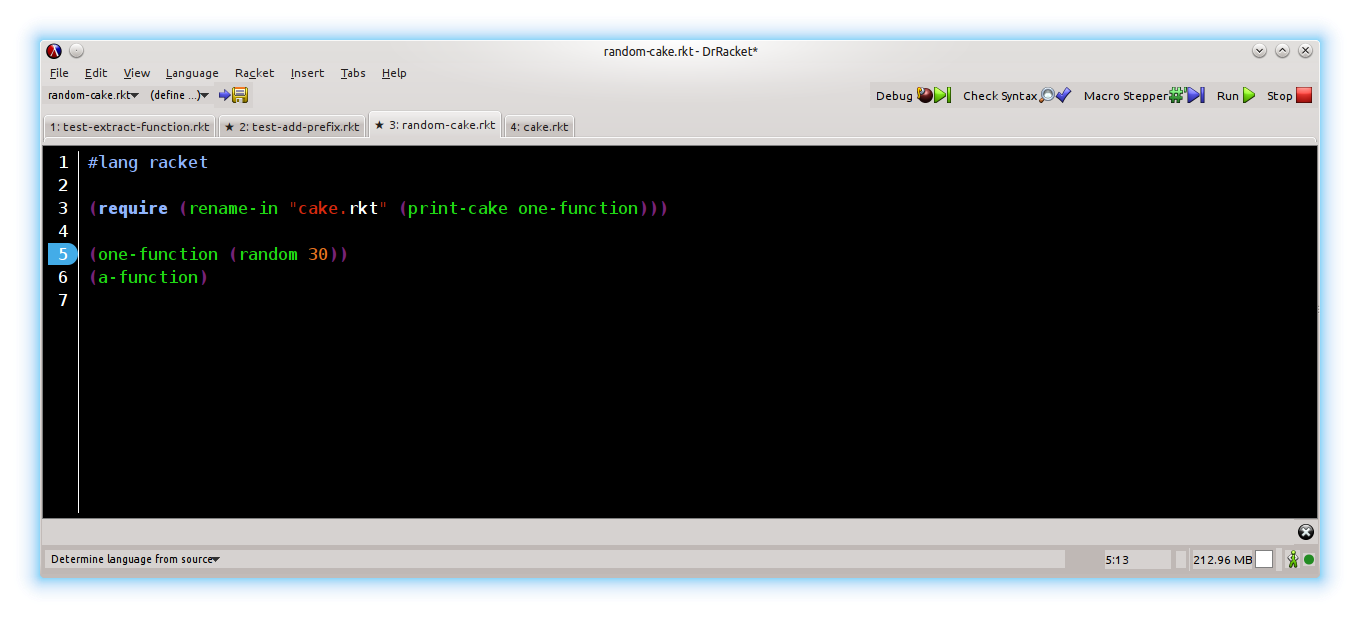
\includegraphics[width=0.95\textwidth]{img/rename2.png}
	\caption{After the Rename}
	\label{fig:renameAfter}
\end{figure}

\subsubsection{Add-prefix}

This is a particular refactoring operation for Racket. Adding a prefix is usually used when there is naming conflicts with two different libraries. The user goes to the library name, and add a prefix.
In the {\bf Figure~\ref{fig:addPrefixBefore}} the arrows show which functions belong to the ``pict3d'' library.
Then the user selects a name for the prefix that will be added, as shown in {\bf Figure~\ref{fig:addPrefixDuring}}. The final result is shown in {\bf Figure~\ref{fig:addPrefixAfter}}.

\begin{figure}[htbp]
	\centering
	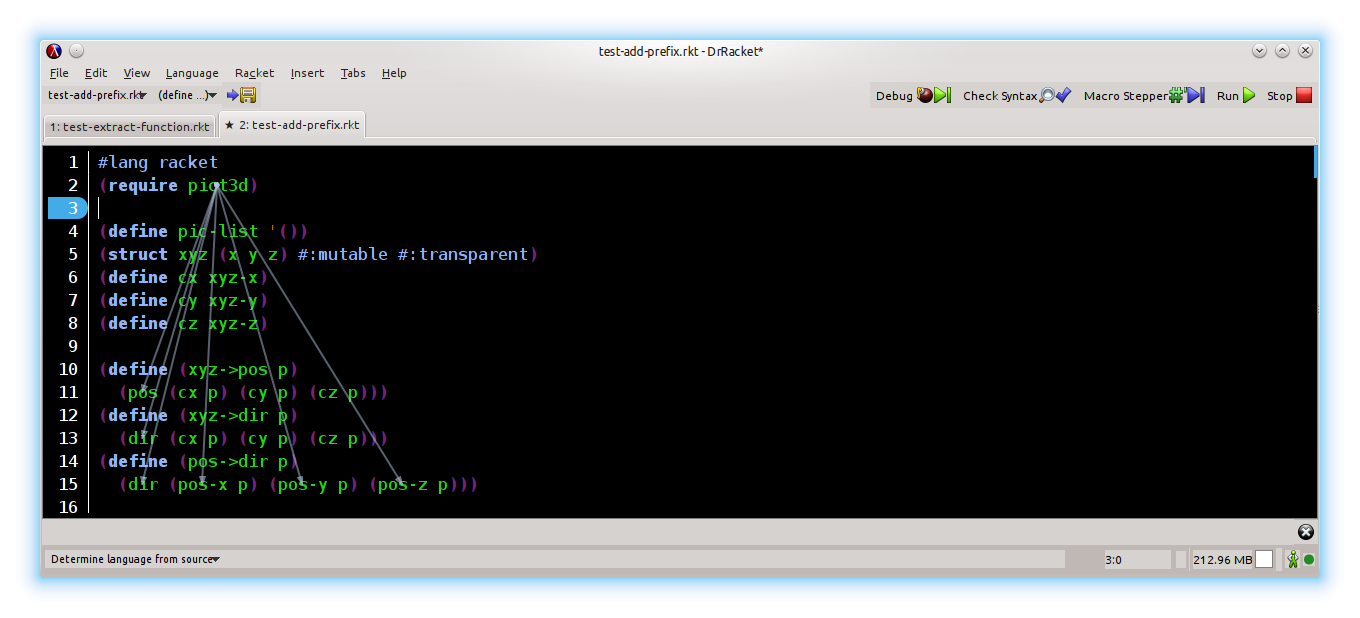
\includegraphics[width=0.95\textwidth]{img/add-prefix.png}
	\caption{Before adding the prefix}
	\label{fig:addPrefixBefore}
\end{figure}

\begin{figure}[htbp]
	\centering
	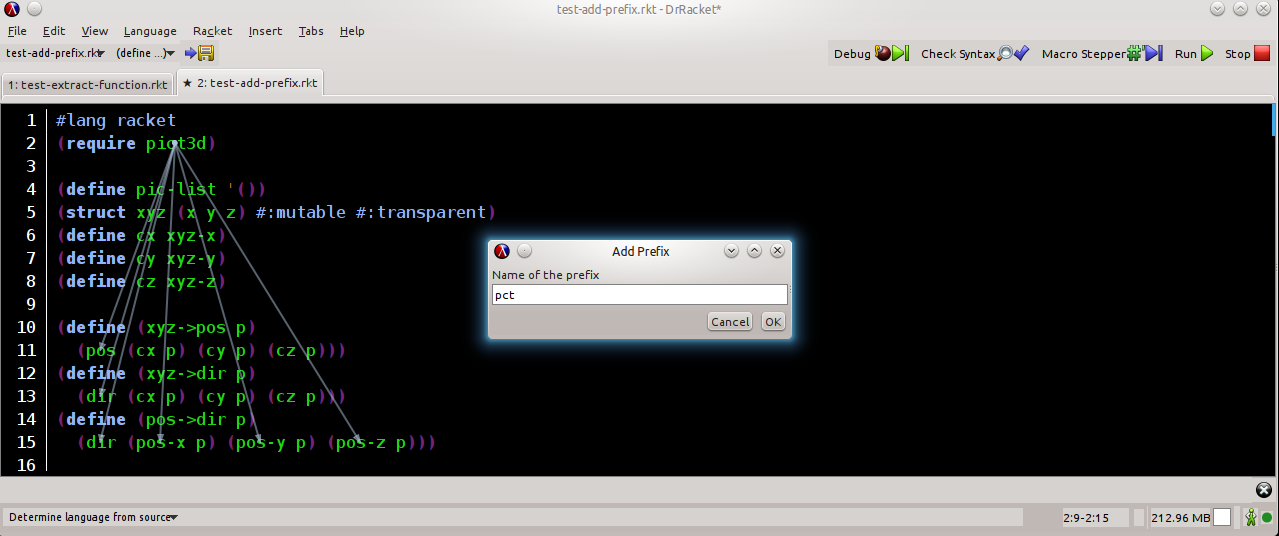
\includegraphics[width=0.95\textwidth]{img/add-prefix1.png}
	\caption{Choosing the prefix}
	\label{fig:addPrefixDuring}
\end{figure}

\begin{figure}[htbp]
	\centering
	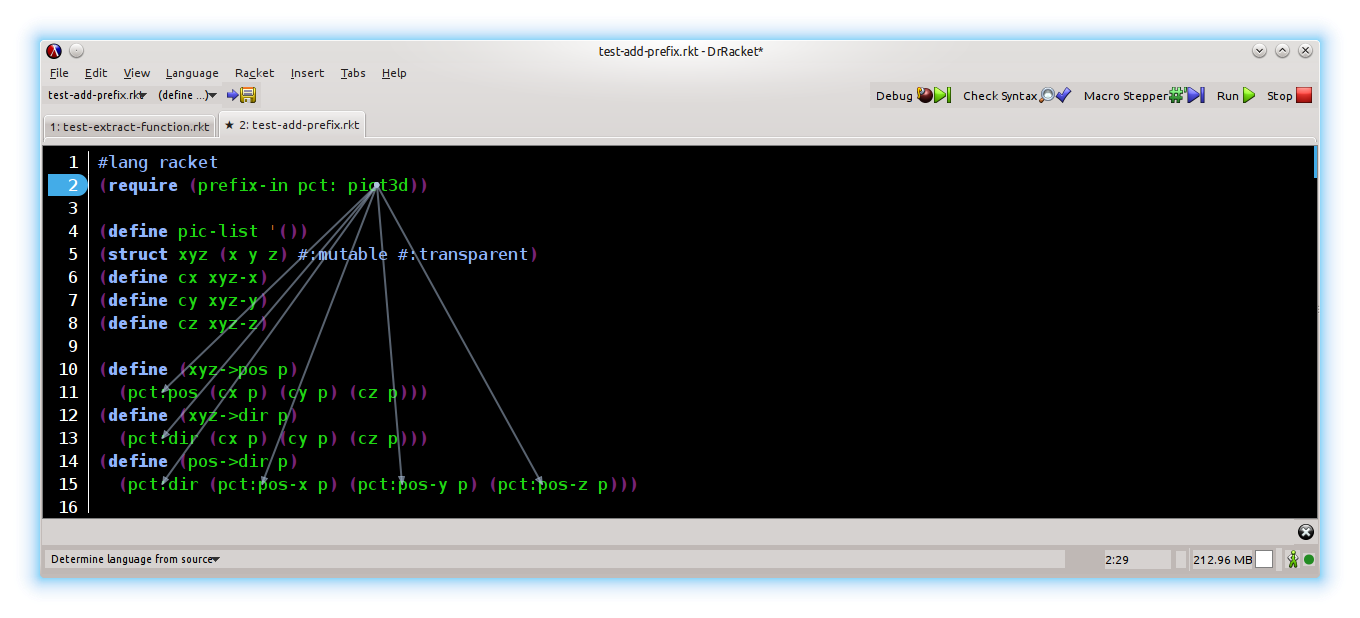
\includegraphics[width=0.95\textwidth]{img/add-prefix2.png}
	\caption{After the Add-prefix refactoring}
	\label{fig:addPrefixAfter}
\end{figure}